\documentclass{article}

% NeurIPS 2025 style (vendored in neurips/neurips_2025.sty), preprint mode:
% these are self-study reports, not conference submissions.
\PassOptionsToPackage{numbers,sort&compress}{natbib}
\usepackage[preprint]{neurips/neurips_2025}

\usepackage[T1]{fontenc}
\usepackage{amsmath,amssymb}
\usepackage{booktabs}
\usepackage{graphicx}
\usepackage{array}
\usepackage[table]{xcolor}
\usepackage{tikz}
\usetikzlibrary{positioning,arrows.meta}
\usepackage[colorlinks=true,linkcolor=blue,urlcolor=blue,citecolor=blue]{hyperref}

% Okabe-Ito-derived palette: status is always paired with a written label,
% never carried by color alone.
\definecolor{nativecol}{HTML}{0072B2}
\definecolor{genericcol}{HTML}{009E73}
\definecolor{partcol}{HTML}{E69F00}
\definecolor{unattcol}{HTML}{D55E00}

\newcolumntype{L}[1]{>{\raggedright\arraybackslash}p{#1}}
% neurips_2025 preprint mode does not update \textwidth (see the geometry
% \newgeometry caveat in neurips_2025.sty), so column widths are literal.
\newlength{\dimcol}\setlength{\dimcol}{3.7cm}
\newlength{\lblcol}\setlength{\lblcol}{1.9cm}

\newcommand{\codex}[0]{Codex}
\newcommand{\occ}[0]{OpenCode}
\newcommand{\ccc}[0]{Claude Code}

\title{Claude Code, Codex, and OpenCode with Open-Source Models:\\
A Static Compatibility Trace}
\author{self-study-with-ai}
\date{\today}

\begin{document}
\maketitle

\begin{abstract}
We ask how three production coding agents, \ccc{}, \codex{}, and
\occ{}, support open-source models, and trace the answer statically:
pinned repositories, official documentation snapshots, no execution.
The three answers divide cleanly. \codex{} ships native Ollama and LM
Studio provider entries that speak OpenAI's Responses API against
localhost servers, with an Ollama version probe that rejects reported
versions older than 0.13.4, and defaults to the gpt-oss family, at the
cost of its patch tool, which is not registered for those models. \occ{} supports any OpenAI-compatible
endpoint through a generic provider path (base URL configuration,
runtime-installed SDKs, a hosted model catalog), but its config defaults
leave unknown models with a zero context limit, which silently disables
auto-compaction, and a zero output limit, which silently becomes a
32{,}000-token request. \ccc{} documents no open-model surface at all: its documented paths are
Anthropic-model clouds, and its closest escape hatches (an unvalidated
base-URL pass-through and capability overrides) are gray-zone mechanisms
whose wire behavior is nowhere attested. A server-side compatibility bar
falls out of the reference servers: chat completions with tool calling
is the practical minimum, Responses API support is partial or
conversion-shaped, and an Anthropic messages route documented by
llama.cpp and an Anthropic-compatible surface named by LM Studio both sit
unverified against \ccc{}. All findings are
bounded to the pinned commits (\path{af70018}, \path{d545d8f},
\path{c3d2e35}) and the documentation snapshots of 2026-08-20.
\end{abstract}

\section{Introduction}

A coding agent with a closed model list is a product; a coding agent
that can run against a local model is a platform. Whether a given
harness supports open-source models is a concrete, answerable question:
does the provider plumbing know about local servers, what wire protocol
does it speak, and what degrades when the model on the other end is not
the vendor's own? We answer it for three systems studied in our harness
comparison, \ccc{}, \codex{}, and \occ{}, at the same pinned commits
(\path{af70018}, \path{d545d8f},
\path{c3d2e35})~\citep{codexRepo,opencodeRepo,claudeCodeSurface}.

The compatibility question has three surfaces to hold constant while the
agent varies: Ollama, LM Studio, and the generic OpenAI-compatible
server class embodied by the llama.cpp reference
server~\citep{ollamaCompatDocs,lmstudioApiDocs,llamaCppServerDocs}. We
also ask the mirror question: what must a compatible server provide for
an agent to survive against it?

This briefing is a static source trace. Nothing was executed, no model
API was called, and provider behavior is stated only as code paths and
documentation contracts. Where a system's behavior is closed or
unattested, the cell says so (Section~\ref{sec:limitations}).

\section{Method and Sources}
\label{sec:methods}

Three local checkouts, the same commits as the harness study, were
pinned for this study on 2026-08-20 at commits
\path{af700180808cce2ce28a31aad0fbad4dc58b857a} (\codex{}, Apache-2.0),
\path{d545d8fba57283528db69281f59c803c646eb7e9} (\occ{}, MIT,
\texttt{dev} branch), and
\path{c3d2e35e554060b5a20ee6b28140fbdbd4eb0048}
(\ccc{})~\citep{codexRepo,opencodeRepo,claudeCodeSurface}. Provider
plumbing was traced in the pinned trees (dedicated \codex{} Ollama and LM
Studio crates; \occ{}'s provider module); \ccc{}'s loader is closed, so
its column is filled from documentation snapshots fetched 2026-08-20
(model configuration and Amazon
Bedrock)~\citep{claudeCodeModelDocs,claudeCodeBedrockDocs}. The
server-side contract was traced in the reference servers' own
documentation: the 2024 Ollama OpenAI-compatibility
post~\citep{ollamaCompatDocs}, LM Studio's developer docs (snapshotted
via its public docs repository, because the live site was unreachable
from the study environment)~\citep{lmstudioApiDocs}, and the llama.cpp
server README at master~\citep{llamaCppServerDocs}. One community
router for \ccc{} was admitted at context tier only, hedged throughout;
it fills no compatibility cell~\citep{claudeCodeRouterContext}.

Prior understanding from the harness study was reused as orientation
only~\citep{codexRepo,opencodeRepo}: every claim here carries its own
anchor in this study's notes (3 codebase notes, 7 documentation notes,
1 context note).

\section{Findings}

\subsection{What the servers themselves provide}
\label{sec:servers}

The compatibility bar is set by what a compatible server can actually
do (Table~\ref{tab:servers}, Figure~\ref{fig:protocolbar}).

\begin{table}[t]
\centering
\small
\caption{Server-side contract, from each reference server's own
documentation snapshots. Responses: whether an OpenAI Responses API
route exists and how it is described.}
\label{tab:servers}
\setlength{\tabcolsep}{4pt}%
\begin{tabular}{@{}L{1.7cm}L{3.9cm}L{3.9cm}L{3.5cm}@{}}
\toprule
Server & Baseline OpenAI surface & Tool calling & Responses API\\
\midrule
Ollama (2024 post) & \path{/v1/chat/completions} at \path{localhost:11434}; auth placeholder ``required, but unused'' (\texttt{ollama\-Compat\-Docs}) & listed as a possible future improvement at post time & not mentioned\\
LM Studio & chat completions and more at \path{localhost:1234/v1} (\path{lmstudio\-Api\-Docs}) & on \path{/v1/chat/completions}; parallel calls and \path{tool_choice} undocumented; streaming deltas indexed & route exists; docs cover streaming, \path{reasoning.effort}, \path{previous_response_id}, remote MCP tools; no function tools documented on that page\\
llama.cpp reference server & models, completions, chat completions, embeddings, plus health, props, metrics, slots; self-described: ``no strong claims of compatibility'' & template-gated via \path{--jinja}; \path{parallel_tool_calls} ``only supported on some models'' & exists but is a converter stub into chat completions; no streaming or tools documented for the route\\
\bottomrule
\end{tabular}
\end{table}

\begin{figure}[t]
\centering
\begin{tikzpicture}[font=\scriptsize, scale=0.92, transform shape,
  proto/.style={draw=black!70, line width=0.7pt, rounded corners=1pt,
    fill=black!5, align=center, minimum width=3.85cm, minimum height=0.95cm,
    inner sep=2.5pt, text=black},
  reqlab/.style={draw=black!40, line width=0.5pt, rounded corners=1pt,
    align=center, minimum width=3.85cm, minimum height=0.85cm,
    inner sep=2.5pt, text=black},
  chip/.style={rounded corners=1pt, align=center, minimum width=3.85cm,
    minimum height=0.85cm, inner sep=2.5pt, text=black},
  rowhead/.style={draw=black!50, line width=0.5pt, rounded corners=1pt,
    fill=black!5, align=center, minimum width=2.3cm, inner sep=2.5pt,
    text=black},
  arr/.style={-{Stealth[length=1.8mm]}, draw=black!60, line width=0.5pt}]
% protocol columns
\node[proto] (p1) at (0,0) {\textbf{Chat completions}\\ plus tool calls};
\node[proto] (p2) at (4.25,0) {\textbf{Responses API}\\ (OpenAI)};
\node[proto] (p3) at (8.5,0) {\textbf{Anthropic}\\ \path{/v1/messages}};
% agent requirements
\node[reqlab, fill=genericcol!14] (oc) at (0,1.75) {\occ{} accepts any\\ chat-completions shape};
\node[reqlab, fill=nativecol!14] (cx) at (4.25,1.75) {\codex{} pins Responses;\\ \path{chat} is a hard error};
\node[reqlab, fill=unattcol!14] (ccreq) at (8.5,1.75) {\ccc{}: Anthropic protocol\\ only, as attested};
\draw[arr] (oc.south) -- (p1.north);
\draw[arr] (cx.south) -- (p2.north);
% Ollama row
\node[rowhead] at (-3.0,-1.4) {Ollama\\ 2024 snapshot};
\node[chip, fill=partcol!16] at (0,-1.4) {partial: chat yes, tools\\ listed as future};
\node[chip, fill=black!7] at (4.25,-1.4) {absent: not in snapshot};
\node[chip, fill=black!7] at (8.5,-1.4) {absent: not in snapshot};
% LM Studio row
\node[rowhead] at (-3.0,-2.5) {LM Studio\\ docs mirror};
\node[chip, fill=genericcol!14] at (0,-2.5) {supported: tools on chat\\ completions; no parallel flag};
\node[chip, fill=partcol!16] at (4.25,-2.5) {partial: streaming, effort,\\ prior state, remote MCP only};
\node[chip, fill=black!7] at (8.5,-2.5) {named only: shape\\ undocumented};
% llama.cpp row
\node[rowhead] at (-3.0,-3.6) {llama.cpp\\ reference server};
\node[chip, fill=genericcol!14] at (0,-3.6) {supported: tools via\\ jinja templates, JSON schema};
\node[chip, fill=partcol!16] at (4.25,-3.6) {partial: documented as a\\ converter to chat completions};
\node[chip, fill=genericcol!14] at (8.5,-3.6) {supported:\\ \path{/v1/messages} documented};
\end{tikzpicture}
\caption{Wire protocols as a compatibility bar. Top row: the protocol each
agent commits to. Bottom grid: what each reference server documents for
that protocol. Every status is written into its chip; shading only
repeats the status.}
\label{fig:protocolbar}
\end{figure}

Two readings matter for the agents. First, the practical minimum for a
coding agent is chat completions with tool calling; streaming is a
comfort feature, and structured output support is uneven. Second, the
Responses API surface is young and incomplete everywhere it exists: an
agent that pins itself to Responses (Section~\ref{sec:codex}) is betting
on servers catching up. A separate fact becomes relevant in
Section~\ref{sec:ccc}: the llama.cpp reference server also exposes an
Anthropic-shaped \path{/v1/messages} route, and LM Studio documents an
Anthropic-compatible surface~\citep{llamaCppServerDocs,lmstudioApiDocs}.

\subsection{Codex: a first-class Responses path, with caveats}
\label{sec:codex}

\codex{}'s answer is structural: Ollama and LM Studio are not generic
endpoints bolted on, they are provider entries. Both are registered with
the responses wire type, and all model traffic is
\path{POST <base_url>/responses}, \path{http://localhost:11434/v1/responses}
and \path{http://localhost:1234/v1/responses}
(\path{codex-rs/model-provider-info/src/lib.rs:514-521},
\path{codex-rs/codex-api/src/endpoint/responses.rs:100-102}). The
legacy chat wire is not a fallback: setting \path{wire_api = "chat"} is a
hard deserialization error~\citep{codexRepo}.

Three design details shape the experience. \emph{Version gating}: before
use, \codex{} probes Ollama with \path{GET /api/version} and refuses
servers that report a version older than 0.13.4, except dev builds that
report \path{0.0.0} and servers whose version endpoint is missing or
unparsable; the gate is consistent with Responses support landing in
later Ollama releases, although the code does not state the
reason~\citep{codexRepo,ollamaCompatDocs}. \emph{Logistics}: the LM
Studio client probes \path{GET <base>/models}, downloads via
\path{lms get --yes}, and warms up with a one-token responses request;
the Ollama client pulls models over the native \path{/api/pull} NDJSON
stream, reading success from the event stream rather than the HTTP
status~\citep{codexRepo}. \emph{Defaults}: the default models are
\path{gpt-oss:20b} (Ollama) and \path{openai/gpt-oss-20b} (LM Studio),
slugs from the gpt-oss open-weight family~\citep{codexRepo}.

The caveats are equally structural. Those default slugs are absent from
the bundled catalog, so, provided the catalog refresh does not decode a
richer listing from the server, they resolve to a fallback model
description with no patch tool type, and the \path{apply_patch} tool is
registered only when that type is set: open models on \codex{} lose the
patch tool, while the rest of the registry is gated by feature and
environment rather than provider~\citep{codexRepo}. Requests to local
servers still carry the full field set, tools JSON,
\path{tool_choice: "auto"}, \path{parallel_tool_calls}, schema-shaped
output, \path{reasoning.summary} defaulting to auto, and
\texttt{include: ["reasoning.encrypted\_content"]}; the server-side
acceptance of each field is not checkable from either side of this
trace~\citep{codexRepo,lmstudioApiDocs,llamaCppServerDocs}. Unknown
models inherit, under the same fallback proviso, a context accounting
of 272{,}000 tokens unless the user sets
\path{model\_context\_window}, and overrides exist via
\path{CODEX\_OSS\_BASE\_URL} and \path{CODEX\_OSS\_PORT}; no OSS provider
entry carries authentication~\citep{codexRepo}.

\subsection{OpenCode: generic compatibility, permissive defaults}
\label{sec:opencode}

\occ{} has the widest answer and the sharpest degradations. Any provider
it does not know rides the generic OpenAI-compatible SDK: the factory is
one of 24 bundled provider packages and is also the final fallback for
catalog models and config-defined
models~\citep{opencodeRepo}. The user-facing shape is a config
block, \path{provider.<id>} with \path{options.baseURL} and
\path{options.apiKey} plus per-model limits; an in-repo test example
runs exactly the Ollama setup, \path{baseURL "http://localhost:11434/v1"}
with limits context 8192, output 2048. Custom SDKs install at runtime
from \path{npm}, or from a local path via \path{file://}, and the hosted
catalog at models.opencode.ai (five-minute cache, overridable and
disablable by flags) lists, in the pinned test fixture, an
\path{lmstudio} provider at \path{http://127.0.0.1:1234/v1} and an
\path{ollama-cloud} provider, though no bare local Ollama
entry~\citep{opencodeRepo}.

The degradations follow from the defaults. An unconfigured limit is
zero: output limit zero silently becomes the 32{,}000-token request cap
(\path{OUTPUT\_TOKEN\_MAX}), and context limit zero disables
auto-compaction entirely, so a local session can drive straight into the
wall without the harness budgeting anything~\citep{opencodeRepo}. Token
counts for unknown models are estimated as characters over four; the
compaction reserve on the v1 overflow path, when it runs, is
min(20{,}000 tokens, \path{maxOutputTokens}); a second compaction path
exists in the pinned tree and which one serves the default run is
unresolved~\citep{opencodeRepo}. Tools are sent unconditionally with the
capability flag defaulting to true, so a server without tool support is
not discovered until the request fails, or, worse, the model simply
never calls a tool and file editing quietly
disappears~\citep{opencodeRepo}. An unknown model string is a hard error
with fuzzy suggestions rather than a silent fallback, which is honest but
unforgiving~\citep{opencodeRepo}. Two filters shape what open models
see: \path{websearch} is dropped for every provider except the native
ones, and the model-ID-keyed choice is the edit path, the
\path{apply\_patch} port is gated to model IDs containing \path{gpt-},
excluding \path{gpt-4} and \path{oss}, so open models get the
\path{edit} and \path{write} tools instead~\citep{opencodeRepo}.

\subsection{Claude Code: no documented surface, and a gray zone}
\label{sec:ccc}

The documentation snapshots are unambiguous about what is supported:
Anthropic-model clouds. The model page covers aliases, version pins, and
provider-specific resolution across Anthropic's own infrastructure,
Bedrock, Google's Agent Platform, and partner clouds, and the Bedrock
page wires Claude Code to AWS with \path{CLAUDE\_CODE\_USE\_BEDROCK=1};
every documented model example there is an Anthropic model, IDs prefixed
or namespaced \path{anthropic.} plus inference-profile
ARNs~\citep{claudeCodeModelDocs,claudeCodeBedrockDocs}. Neither snapshot
mentions Ollama, LM Studio, open-weight models, or an OpenAI-compatible
endpoint anywhere (verified absence).

The gray zone is three documented mechanisms whose intended use is not
open models but whose wording leaves a gap. \path{ANTHROPIC\_BASE\_URL}
``changes where requests are sent, not which model answers them'', and
behind a custom base URL the client ``passes any string through without
checking it''; \path{ANTHROPIC\_CUSTOM\_MODEL\_OPTION} adds an
unvalidated picker entry (``you can use any string your API endpoint
accepts''); and \path{CLAUDE\_CODE\_MAX\_CONTEXT\_TOKENS} applies to
model IDs that do not start with \path{claude-}, do not carry the
\path{[1m]} marker, and do not resolve to a Claude
model~\citep{claudeCodeModelDocs}.
Capability gating is model-ID-shaped with override variables, and
context-window enforcement for unknown IDs can be deferred to the
server's too-long error, a mode documented as failing ``when a gateway
rewrites the error''~\citep{claudeCodeModelDocs}. Whether an
Anthropic-protocol server can actually drive a session is unattested in
every source this study registered; the llama.cpp reference server
documents an Anthropic messages route and LM Studio names an
Anthropic-compatible surface, both unverified against \ccc{}, which makes
the gap worth stating explicitly rather than
closing~\citep{llamaCppServerDocs,lmstudioApiDocs}.
A community router claims to bridge \ccc{} to a long list of providers
from a local gateway, but the claim is self-reported, never names Ollama
or LM Studio, and is held at context tier~\citep{claudeCodeRouterContext}.

\subsection{The matrix}
\label{sec:matrix}

\begin{table}[t]
\centering
\small
\caption{Compatibility matrix at the pinned commits. Tier: native means
dedicated provider code in the agent; generic means a config-driven
compatible-endpoint path; none means no documented surface. Caveats
abbreviate Section~\ref{sec:servers} to~\ref{sec:ccc}.}
\label{tab:matrix}
\setlength{\tabcolsep}{4pt}%
\begin{tabular}{@{}L{1.7cm}L{4.0cm}L{4.0cm}L{3.3cm}@{}}
\toprule
Agent & Ollama & LM Studio & Generic server\\
\midrule
\cellcolor{nativecol!10}\codex{} & native, Responses wire, port 11434, refuses reported versions below 0.13.4, default \path{gpt-oss:20b} & native, Responses wire, port 1234, default \path{openai/gpt-oss-20b}, model pull via \path{lms} & via \path{model_providers} config, Responses wire only; \path{chat} is a hard error\\
\cellcolor{genericcol!10}\occ{} & config-defined generic path; in-repo example \path{localhost:11434/v1}; catalog lists only \path{ollama-cloud} & generic path; catalog fixture at \path{127.0.0.1:1234/v1} & \path{@ai-sdk/openai-compatible} fallback; base URL config; runtime SDK install\\
\cellcolor{unattcol!8}\ccc{} & none documented; base-URL pass-through is gray zone & none documented; same gray zone & none documented; Anthropic protocol only; gateway wire shape unattested\\
\bottomrule
\end{tabular}
\end{table}

\begin{figure}[t]
\centering
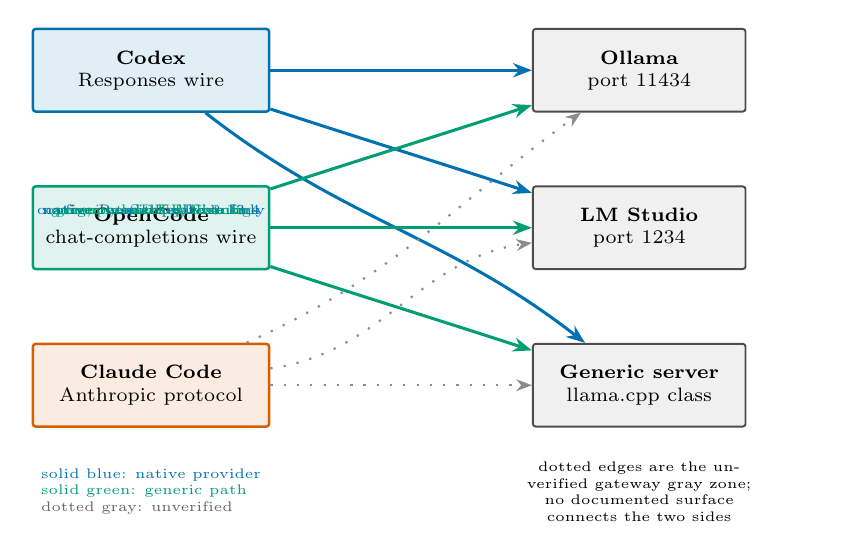
\begin{tikzpicture}[font=\scriptsize,
  agent/.style={draw=#1, line width=0.9pt, rounded corners=1pt, fill=#1!12,
    text=black, minimum width=3.0cm, minimum height=1.05cm, align=center},
  server/.style={draw=black!70, line width=0.7pt, rounded corners=1pt,
    fill=black!6, text=black, minimum width=2.7cm, minimum height=1.05cm,
    align=center},
  nat/.style={-{Stealth[length=2.4mm]}, line width=1.1pt, nativecol},
  gen/.style={-{Stealth[length=2.4mm]}, line width=1.1pt, genericcol},
  unv/.style={-{Stealth[length=2mm]}, line width=0.8pt, black!45, loosely dotted}]
% agents
\node[agent=nativecol] (cx) at (0, 2.0) {\textbf{Codex}\\ Responses wire};
\node[agent=genericcol] (oc) at (0, 0.0) {\textbf{OpenCode}\\ chat-completions wire};
\node[agent=unattcol] (cc) at (0,-2.0) {\textbf{Claude Code}\\ Anthropic protocol};
% servers
\node[server] (ol) at (6.2, 2.0) {\textbf{Ollama}\\ port 11434};
\node[server] (lm) at (6.2, 0.0) {\textbf{LM Studio}\\ port 1234};
\node[server] (gn) at (6.2,-2.0) {\textbf{Generic server}\\ llama.cpp class};
% Codex edges
\draw[nat] (cx) to[out=0, in=180] (ol)
  node[sloped, midway, above, font=\tiny, text=nativecol, pos=0.5] {native; version gate 0.13.4};
\draw[nat] (cx) to[out=-18, in=162] (lm)
  node[sloped, midway, above, font=\tiny, text=nativecol, pos=0.52] {native; model pull via lms};
\draw[nat] (cx) to[out=-38, in=142] (gn)
  node[sloped, midway, above, font=\tiny, text=nativecol, pos=0.58] {config; Responses wire only};
% OpenCode edges
\draw[gen] (oc) to[out=18, in=198] (ol)
  node[sloped, midway, above, font=\tiny, text=genericcol, pos=0.48] {generic; baseURL config};
\draw[gen] (oc) to[out=0, in=180] (lm)
  node[sloped, midway, above, font=\tiny, text=genericcol, pos=0.5] {generic; catalog fixture};
\draw[gen] (oc) to[out=-18, in=162] (gn)
  node[sloped, midway, above, font=\tiny, text=genericcol, pos=0.52] {compat-SDK fallback};
% Claude Code edges: unverified gray zone
\draw[unv] (cc) to[out=24, in=216] (ol);
\draw[unv] (cc) to[out=8, in=188] (lm);
\draw[unv] (cc) to[out=0, in=180] (gn);
\node[align=center, font=\tiny, text width=4.6cm] at (6.2,-3.35)
  {dotted edges are the unverified gateway gray zone;\\ no documented surface connects the two sides};
\node[align=left, font=\tiny] at (0,-3.35)
  {\textcolor{nativecol}{solid blue: native provider}\\
   \textcolor{genericcol}{solid green: generic path}\\
   \textcolor{black!60}{dotted gray: unverified}};
\end{tikzpicture}
\caption{Support as a graph. Solid arrows are attested paths with their
tier; dotted arrows mark the \ccc{} gray zone where no source attests the
connection. Values match Table~\ref{tab:matrix}.}
\label{fig:support}
\end{figure}

Read together, the matrix, the caveats, and Figure~\ref{fig:support}
support one directional claim:
compatibility with open models is decided by the wire protocol an agent
commits to. \codex{} committed to Responses and built native plumbing
for two local servers, accepting the patch-tool loss and betting on
server-side adoption. \occ{} committed to nothing and accepts anything
chat-completions-shaped, accepting that its accounting defaults misbehave
around zero limits. \ccc{} commits to Anthropic's stack and leaves the
rest to whatever the user can route through a gateway, unattested.

\section{Related Work}
\label{sec:related}

The nearest verifiable work is our own static comparison of these three
harnesses, which established the eight-dimension decomposition and
traced the configuration and provider dimension at the same
pins~\citep{codexRepo,opencodeRepo,claudeCodeSurface}. This briefing
narrows that dimension's provider half to the open-model question and
adds the server-side contract from the reference servers'
documentation~\citep{ollamaCompatDocs,lmstudioApiDocs,%
llamaCppServerDocs}, which the harness study did not cover. It differs
from ordinary compatibility reports in one respect: it reports no
behavior, because none was measured; every cell is a code path, a
documentation contract, or a labeled gap. The community router around
\ccc{} sits in the nearest-work neighborhood as an existence proof that
users route around the closed loader, not as
evidence~\citep{claudeCodeRouterContext}.

\section{Limitations}
\label{sec:limitations}

\paragraph{No behavior was measured.} This is the briefing's governing
constraint: no agent ran, no server served, no model answered. Every
compatibility statement is a contract statement. Server acceptance of
agent request fields (tools JSON, parallel calls, reasoning fields) is
the single largest uncheckable cell and is marked as such in the
notes~\citep{codexRepo,lmstudioApiDocs}.

\paragraph{Version and provenance bounds.} Findings are bounded to three
pinned commits and snapshots fetched 2026-08-20. The Ollama snapshot is
the 2024 compatibility post, which predates the version \codex{}
requires; current Ollama behavior beyond that gate is not covered. LM
Studio snapshots came from its documentation repository because the live
site was unreachable from the study environment, so drift from the
shipped application is unassessed. The llama.cpp snapshot is master at
fetch time, unversioned. vLLM's compatible-server documentation moved
and could not be re-located within budget, so the generic bar is carried
by llama.cpp and LM Studio alone~\citep{ollamaCompatDocs,lmstudioApiDocs,%
llamaCppServerDocs}.

\paragraph{Closed core.} \ccc{}'s loader is closed; its column is
documentation-attested or negative scope. The wire shape of its gateway
traffic is nowhere attested, which means both the pass-through mechanism
and any Anthropic-compatible-server hypothesis are uncheckable
here~\citep{claudeCodeModelDocs,claudeCodeBedrockDocs}.

\paragraph{Catalog state.} \occ{}'s live model catalog is runtime state;
only the pinned test fixture is inspectable, so claims about catalog
contents are fixture-scoped~\citep{opencodeRepo}.

\paragraph{Codex fallback metadata.} The patch-tool loss and the
272{,}000-token accounting rest on catalog misses resolving to a
fallback description; whether that fallback survives at runtime depends
on the models-catalog refresh decoding against a plain \path{/v1/models}
listing, which expects the rich catalog schema and is not exercised
against a local server in the pinned tree~\citep{codexRepo}.

\paragraph{OpenCode compaction paths.} Two compaction implementations
coexist in the pinned tree, and which one serves the default run was not
traced; the reserve figures here are attributed to the v1 overflow
path~\citep{opencodeRepo}.

\section{Conclusion}

Open-model support is not a setting; it is a wire-protocol decision made
at the architecture level. \codex{} has the deepest first-class support,
via native Responses-API providers for Ollama and LM Studio, at the cost
of the patch tool on those defaults and of unverified field-level
acceptance. \occ{} has the broadest support, any endpoint a base URL can
reach, at the cost of accounting defaults that silently disable
compaction and of a hard fail on unknown model strings. \ccc{} has no
documented open-model path; its gateway mechanisms are a gray zone whose
behavior no source attests, even though the reference servers both speak
its protocol shape at some surface. For a learner choosing today: point \occ{} at anything
OpenAI-compatible after setting context and output limits by hand; run
\codex{} against Ollama 0.13.4 or newer, or LM Studio with gpt-oss
models; and treat \ccc{} with local models as a community-project
problem until the vendor says otherwise. All claims are bounded
to the pinned commits and the snapshots of 2026-08-20.

\bibliographystyle{plainnat}
\bibliography{refs}

\end{document}
